\newpage
\hypertarget{treeToModel vis}{}
\subsection{Vis Tree to Model Source}
\visHeader

\begin{itemize}

\item[$\blacktriangleright$] Be sure to mention how/why do the correspondence type (lock them together, remove a risk, etc etc)
Before running \texttt{TGG.main}, change the instance it looks for from \texttt{box.xmi}\footnote{From Part IV}, to \texttt{tree}.
Be working entirely within the \texttt{DictionaryCodeAdapter} -- drawing classes from \texttt{MocaTree} (parser) and \texttt{DictionaryLanguage}
{\bf update the names of the functions? make them more informative?}


\item[$\blacktriangleright$] already have the basic tgg and one corresp type.

\item[$\blacktriangleright$] First: transform folders:: build \texttt{FolderIntoLibrary}

\begin{figure}[htbp]
\begin{center}
  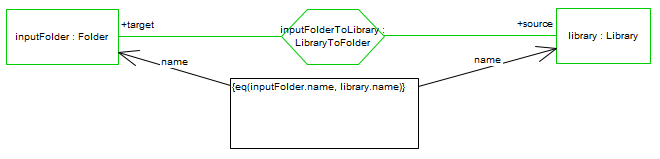
\includegraphics[width=\textwidth]{ea_completeFolderIntoLibrary}
  \caption{completed folder into library}
  \label{ea:FolderIntoLibrary_Complete}
\end{center}
\end{figure}

\item[$\blacktriangleright$] Click each element and \emph{derive} \texttt{ForAllShelves}. We separated here because\ldots This rule therefore now assumes/won't
run unless its invoked in the context of having an inputFolder and library established. This will create a shelf element for every shelf folder it finds in the tree.

\begin{figure}[htbp]
\begin{center}
  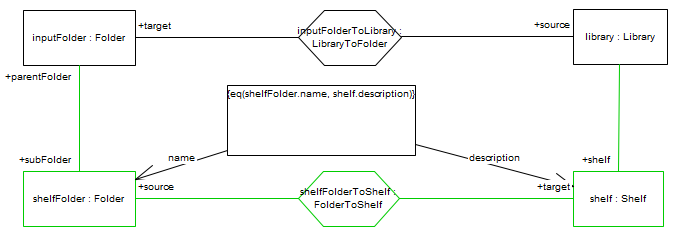
\includegraphics[width=\textwidth]{ea_completeForAllShelves}
  \caption{completed ForAllShelves}
  \label{ea:ForAllShelves_Complete}
\end{center}
\end{figure}

\item[$\blacktriangleright$] Now, we could have included a third, fourth, or tenth node element connected to \texttt{dictionary}, but that would force the
dictionary to have that many elements \emph{every} time. Even if it permitted up to ten, and your tree model only had 9, it would still fail for missing that
final partition.

\begin{figure}[htbp]
\begin{center}
  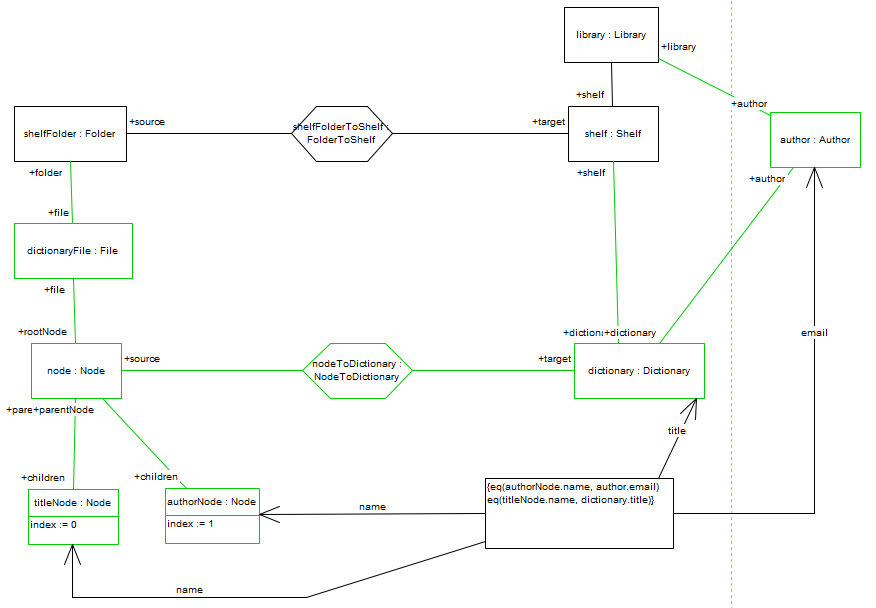
\includegraphics[width=\textwidth]{ea_completeNodeToDictionary}
  \caption{completed NodeToDictionary}
  \label{ea:NodeToDictionary_Complete}
\end{center}
\end{figure}

\item[$\blacktriangleright$] Let's handle the elements below. Similar logic as to \texttt{ForAllShelves} : links and specific context. This is how THAT also
handles multiples.

\begin{figure}[htbp]
\begin{center}
  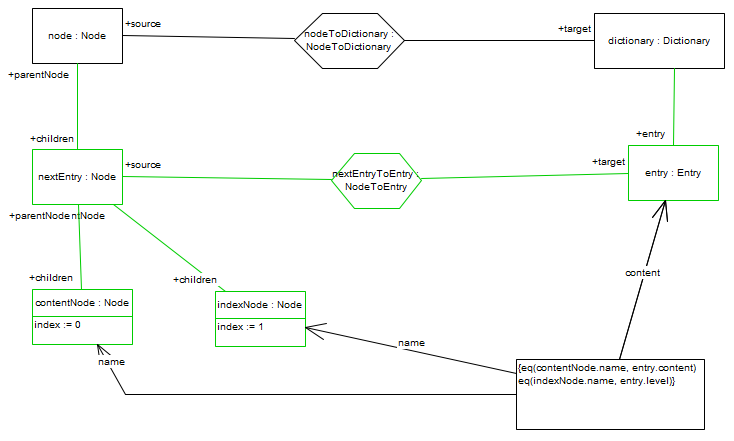
\includegraphics[width=\textwidth]{ea_completeForAllEntry}
  \caption{completed ForAllEntry}
  \label{ea:ForAllEntry_Complete}
\end{center}
\end{figure}

\item[$\blacktriangleright$] Validate: if you're having trouble exporting, try updating your schema first with any missing elements you may have created on the
fly. it should resemble\ldots

\begin{figure}[htbp]
\begin{center}
  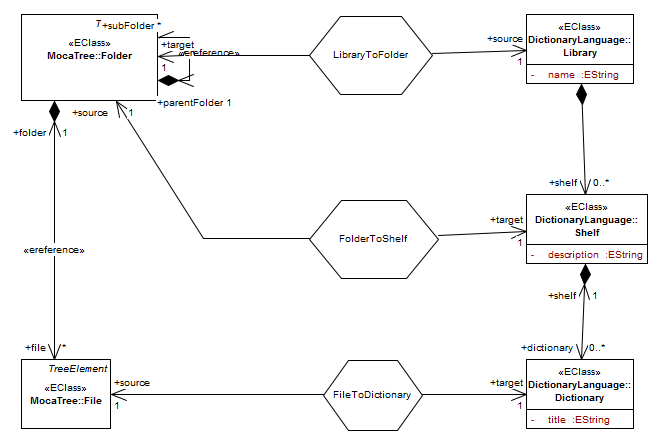
\includegraphics[width=\textwidth]{ea_completeSchema}
  \caption{completed Schema}
  \label{ea:Schema_Complete}
\end{center}
\end{figure}



\end{itemize}


